In order to have a continuous progress, project management had to be established. The goal of it is to ensure that the whole project and software development process works as it is intended, allowing project activities to meet project requirements.
\\
The main steps of project management process are initiating, planning, executing, monitoring and controlling, and closing. Thus firstly, project team meetings were established on a weekly basis. Continuing defining the project goals, tight control of timeline had to be set as well, in order to keep track of deadlines.
\\
For this purpose the Gantt charts web tool\footnote{\url{https://teamgantt.com/}} was employed. It allowed to breakdown work structure of the project to small tasks, setting the start and finish dates individually. Example of Gantt chart used in this project can be seen in figure \ref{fig:gannt_example}.

\begin{figure}[ht!]
	\centering
	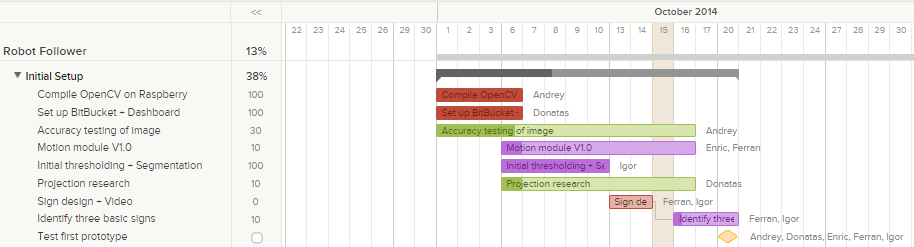
\includegraphics[width=1\textwidth]{gantt_chart_part}
	\caption{Part of planning represented on Gantt chart}
	\label{fig:gannt_example}
\end{figure}

Beside the track of the tasks, version control system for tracking the code changes had to be chosen. Common tools are Team Foundation Version Control, Mercurial or Git source control. Due to affordability and compatibility, distributed version control system Git was chosen. 
\\
For hosting the central GIT repository the two main players are \textit{Github} and \textit{Bitbucket}.
The main difference between the two is being cost for non-open source projects. \textit{Bitbucket} is free for teams up to 5 users and can host private closed source repositories whereas \textit{Github} does not provide private repositories for free. Thus the specifications of providers led to choose \textit{Bitbucket} for being web-based hosting service for this project.
\\
After setting up source version control, actual developing had started. In order to keep track with the Gantt chart, specific issues were created and assigned to each team member on a weekly basis. Project management tool \textit{Bitbucket Cards}, a part of \textit{Bitbucket}, offered interaction with issues on one easy-to-use, intuitive dashboard, where progress of tasks from one list to the next was easy to track.  Example of early stage project board can be seen in figure \ref{fig:bitcards}.

\begin{figure}[ht!]
	\centering
	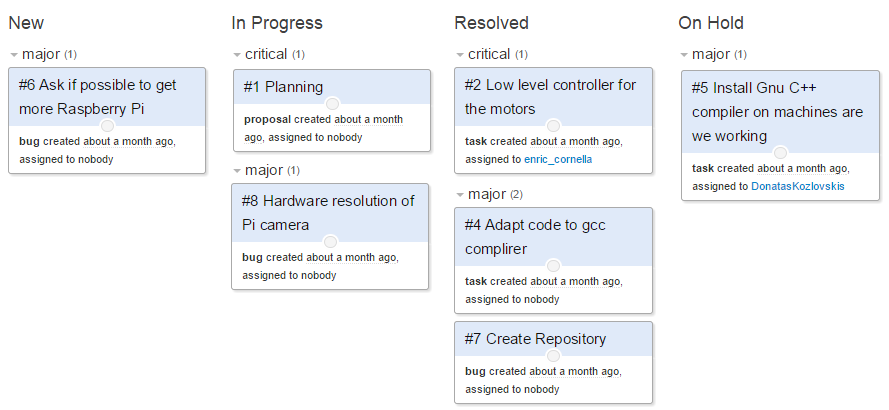
\includegraphics[width=0.7\textwidth]{bitbucket_cards}
	\caption{Early stage project board}
	\label{fig:bitcards}
\end{figure}
